\chapter{Demonstration of the API}

\label{chap:demo}

To get a better understanding of the API and how it works, a demo application was developed. This demo application runs on the web, access the API and demonstrate the capabilities of the API.

\section{Conception}

\label{sec:demo_concept}

The demo application is written with the javascript framework Vue. To handle the requests to the recommendation API we use Axios.

\begin{figure}[h]
\centering
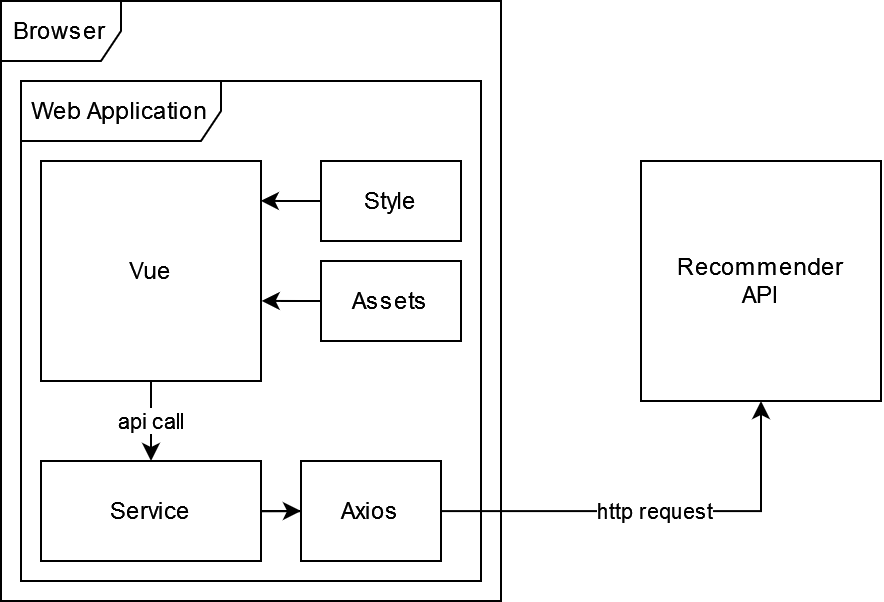
\includegraphics[width=\textwidth]{images/Demo_concept.drawio.png}
\caption{\label{fig:demo_concept}Concept of the Demo Application}
\end{figure}

\newpage

The service in overview \ref{fig:demo_concept} should be an interface or object that contains all possible requests to the API, and should convert the JSON data from the API into Javascript objects.

A UI is created to interact with the demo, the concept is shown in figure \ref{fig:ui_design_demo}.

\begin{figure}[h]
\centering
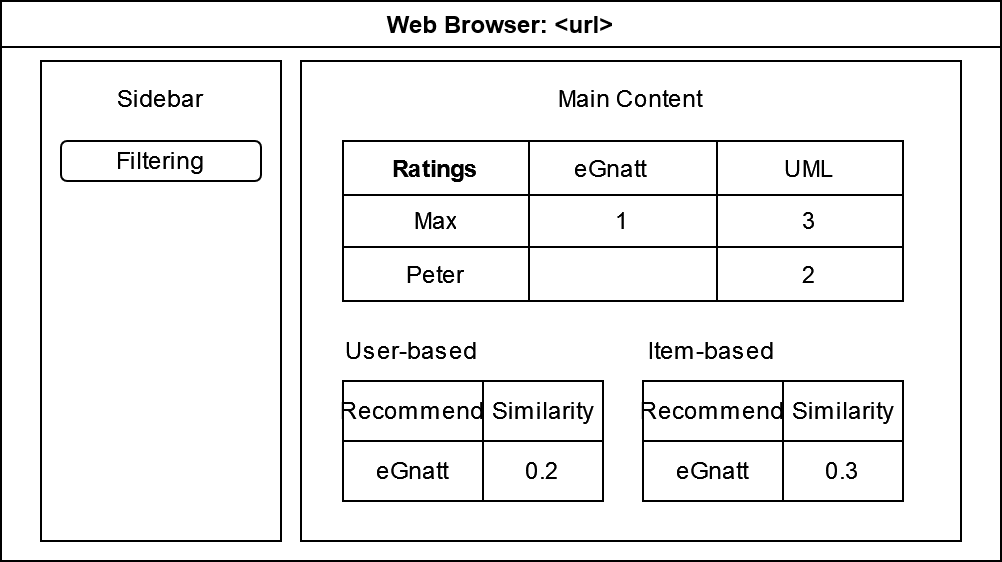
\includegraphics[width=\textwidth]{images/ui_concept.drawio.png}
\caption{\label{fig:ui_design_demo}Concept of the UI}
\end{figure}

\newpage

\section{Technologies}

\label{sec:demo_tec}

We now list the technologies we use in the demo application.

\subsection{Vite}

Vite is a development environment that builds and bundles Javascript, optimised for fast development. Vite addresses certain issues with component-based development and is the recommended build tool for Vue \cite{Vite}.

\subsection{Vue with Typescript}

Vue is a javascript framework that enables the usage of javascript, html and css in components \cite{Vue}. This makes code more reusable and also provides a level of security. Vue also provides plugins such as a router to display components on specific web routes \cite{VueRouter}. Typescript is a strongly typed language that is built on top of JavaScript and is developed and maintained by Microsoft and can also be used for Vue projects \cite{typescirpt}. 

\subsection{Axios}

Axios is an http client that can make xml http requests from the browser. We use Axios to make http requests to the API and convert JSON content to javascript objects.

\section{Implementation}

\label{sec:demo_impl}

Creating a Vue project creates some basic files: The main.ts, App.vue and the components directory. Within the index.ts, we define the Vue router and include styling files such as the base.css file.

\subsection{Router}

As mentioned above, the router is mounted on the application in main.ts and looks like this:

\newpage

\begin{minted}[frame=lines,framesep=2mm,baselinestretch=1.2,fontsize=\footnotesize,bgcolor=LightGray]{ts}
import { createApp } from 'vue'
import './assets/base.scss'
import App from "@/App.vue";
import HomeComponent from "@/components/struc/main/HomeComponent.vue";
import FilteringComponent from "@/components/struc/main/FilteringComponent.vue";
import {createRouter, createWebHashHistory} from "vue-router";
import UserComponent from "@/components/struc/main/UserComponent.vue";
import ItemComponent from "@/components/struc/main/ItemComponent.vue";
import AuthComponent from "@/components/struc/main/AuthComponent.vue";

const routes = [
    { path: '/', component: HomeComponent },
    { path: '/filtering', component: FilteringComponent },
    { path: '/user', component: UserComponent },
    { path: '/items', component: ItemComponent },
    { path: '/authentication', component: AuthComponent },
]

const router = createRouter({
    history: createWebHashHistory(),
    routes,
})

const app = createApp(App)
app.use(router)
app.mount('#app')
\end{minted}

The router allows easy switching between the defined components. Within the sidebar, switching to the routes can be done using buttons.

\subsection{Authentication}

To access the API, a token is required on each request. The demo application manages this by retrieving the token from the user with a text input, and then storing the token as a cookie so that the user is authenticated when they return. 

\begin{minted}[frame=lines,framesep=2mm,baselinestretch=1.2,fontsize=\footnotesize,bgcolor=LightGray]{html}
<script setup lang="ts">
import {ref} from "vue";
const inputToken = ref(localStorage.getItem('token') ?? '')
function save() {
  localStorage.setItem('token', inputToken.value)
}
</script>
<template>
  <div class="main-container">
    <div class="main-header anim" style="--delay: 0s">Authentication</div>
    <div class="input-auth-bar">
      <input v-model="inputToken" type="text" placeholder="Access Token">
      <a @click="save()" class="auth-check">Save</a>
    </div>
  </div>
</template>
\end{minted}

To make API requests with the token easier, a service.ts is defined that retrieves the token and appends it to each request.

\begin{minted}[frame=lines,framesep=2mm,baselinestretch=1.2,fontsize=\footnotesize,bgcolor=LightGray]{ts}
import axios from 'axios'

const API_URL = 'https://bpm.matthiasklenz.de'

const config = {
  baseURL: API_URL,
  timeout: 120000
}

export const service = axios.create(config)

service.interceptors.request.use(async (config) => {
  config.headers!.Authorization = `Bearer ${localStorage.getItem('token')}`
  return config
})

export default service
\end{minted}

\subsection{Filtering View}

The filtering view retrieves all ratings from all users and displays them in a table. To do this, all items are retrieved to show the names of the items.

\begin{minted}[frame=lines,framesep=2mm,baselinestretch=1.2,fontsize=\footnotesize,bgcolor=LightGray]{ts}
export type ItemSimilarity = {
  item: string
  similarity: number
}

export const getAllItems = () => service.get<ItemData[]>('/items')
\end{minted}

All users are retrieved to display the usernames within the table.

\begin{minted}[frame=lines,framesep=2mm,baselinestretch=1.2,fontsize=\footnotesize,bgcolor=LightGray]{ts}
export type UserData = {
  userid: number
  username: string
  info: string | null
}

export const getAllUsers = () => service.get<UserData[]>('/users')
\end{minted}

After the users have been retrieved, the user ratings are retrieved to display them in the table.

\begin{minted}[frame=lines,framesep=2mm,baselinestretch=1.2,fontsize=\footnotesize,bgcolor=LightGray]{ts}
export type UserRating = {
  userid: number
  ratings: Map<number, number>
}

export const getAllUserRatings = () 
    => service.get<UserRating[]>('/user/ratings')
\end{minted}

Once all the information has been retrieved, we can use Vue to create the table with the data provided.

\begin{minted}[frame=lines,framesep=2mm,baselinestretch=1.2,fontsize=\footnotesize,bgcolor=LightGray]{html}
<table>
  <thead>
  <tr>
    <th style="padding-right: 5rem">User</th>
    <th
        v-for="item in items"
        :key="item.id"
        v-on:click="setActiveItem(item.id)"
        v-bind:class="{ active: activeItem === item.id }"
        style="cursor: pointer"
    >
      {{ itemNameWithSimilarity(item.id) }}
    </th>
  </tr>
  </thead>
  <tbody>
    <tr
      v-for="user in userRatings"
      v-bind:class="{ active: activeUser === user.userid }"
      v-bind:key="user.userid"
    >
      <td v-on:click="setActiveUser(user.userid)" style="cursor: pointer">
        {{ usernameWithSimilarity(user.userid) }}
      </td>
      <td v-for="item in items" v-bind:key="item.id">
        {{ user.ratings[item.id.toString()] }}
     </td>
    </tr>
  </tbody>
</table>
\end{minted}

This completes the basic table. We now look at the similarities between users and items. To do this, the usernames and item names are clickable within the table. Clicking on a username will send the following request to the API

\begin{minted}[frame=lines,framesep=2mm,baselinestretch=1.2,fontsize=\footnotesize,bgcolor=LightGray]{ts}
export type UserSimilarity = {
  userid: number
  ratings: Map<number, number>
  similarity: number
}

export const getUserSimilarities = (
    user: number, 
    similarityMeasure: string = 'pearson'
) =>
  service.get<UserSimilarity[]>(
    `/userBased/similarities/${user}?SimilarityMeasure=${similarityMeasure}`
  )
\end{minted}

We can also include a similarity measure when trying to find the similarities between two users. The same can be done when making item similarity queries.

\begin{minted}[frame=lines,framesep=2mm,baselinestretch=1.2,fontsize=\footnotesize,bgcolor=LightGray]{ts}
export type ItemSimilarity = {
  item: string
  similarity: number
}

export const getItemSimilarities = (
    item: number, 
    similarityMeasure: string = 'pearson'
) =>
  service.get<ItemSimilarity[]>(
    `/itemBased/similarities/${item}?SimilarityMeasure=${similarityMeasure}`
  )
\end{minted}

When displaying user similarities, the user-based and item-based recommendations should also be displayed on-screen to show which item is recommended for the current user.


To get the user-based recommendations, we make the following request:

\newpage

\begin{minted}[frame=lines,framesep=2mm,baselinestretch=1.2,fontsize=\footnotesize,bgcolor=LightGray]{ts}
export type EstimatedRecommendations = {
  [key: string]: number
}

export const getUserRecommendations = (
  user: number,
  similarityMeasure: string = 'pearson',
  knn: number = 2,
  weighted: boolean = true
) =>
  service.get<EstimatedRecommendations>(
    `/userBased/recommendations/${user}?SimilarityMeasure=
    ${similarityMeasure}&knn=${knn}&weightedMean=${weighted}`
  )
\end{minted}

A different URL is used for the item-based recommendation:

\begin{minted}[frame=lines,framesep=2mm,baselinestretch=1.2,fontsize=\footnotesize,bgcolor=LightGray]{ts}
export const getItemRecommendations = (
  user: number,
  similarityMeasure: string = 'pearson',
  knn: number = 2,
  weighted: boolean = true
) =>
  service.get<EstimatedRecommendations>(
    `/itemBased/recommendations/${user}?SimilarityMeasure=
    ${similarityMeasure}&knn=${knn}&weightedMean=${weighted}`
  )
\end{minted}

\subsection{User View}

The User View lists all users and their information, users can be added, edited and deleted from the User View. User ratings can also be added in this view.

To add a user, a PUT request with the name and optional information is sent to the API.
\begin{minted}[frame=lines,framesep=2mm,baselinestretch=1.2,fontsize=\footnotesize,bgcolor=LightGray]{ts}
export const addUser = (username: string) 
    => service.put('/user', { username: username })
\end{minted}

To update user information, a UserData object is sent to the API, which then updates the information for the ID within the Data object.

\begin{minted}[frame=lines,framesep=2mm,baselinestretch=1.2,fontsize=\footnotesize,bgcolor=LightGray]{ts}
export const editUser = (userData: UserData) 
    => service.post('/user', userData)
\end{minted}

To delete a user, send a DELETE request with the userid.

\begin{minted}[frame=lines,framesep=2mm,baselinestretch=1.2,fontsize=\footnotesize,bgcolor=LightGray]{ts}
export const delUser = (id: number) => service.delete(`/user/${id}`)
\end{minted}

To add a rating, a POST request is sent with the itemId and userid along with the rating value.

\begin{minted}[frame=lines,framesep=2mm,baselinestretch=1.2,fontsize=\footnotesize,bgcolor=LightGray]{ts}
export const addRating = (userid: number, itemId: number, rating: number) =>
  service.post(
    '/user/rating', 
    { userid: userid, ratings: { [itemId]: rating } }
  )
\end{minted}

\subsection{Item View}

The Item view lists all items with their name and description. The table is structured so that the names and descriptions can be edited, deleted and submitted using a button. To edit an item, an ItemData object is sent and the API updates the entry based on the ID provided in the ItemData object.

\begin{minted}[frame=lines,framesep=2mm,baselinestretch=1.2,fontsize=\footnotesize,bgcolor=LightGray]{ts}
export const editItem = (data: ItemData) => service.post('/item', data)
\end{minted}

To delete an item, all the API needs is the ID.

\begin{minted}[frame=lines,framesep=2mm,baselinestretch=1.2,fontsize=\footnotesize,bgcolor=LightGray]{ts}
export const delItem = (id: number) => service.delete(`/item/${id}`)
\end{minted}

To add a new item, the ItemData is sent as a PUT request without the id.

\begin{minted}[frame=lines,framesep=2mm,baselinestretch=1.2,fontsize=\footnotesize,bgcolor=LightGray]{ts}
export const addItem = (name: string, description: string) =>
  service.put('/item', { name: name, description: description })
\end{minted}
